\section{Výsledky a diskusia}

Numerické výpočty robíme pre kov s Fermiho vlnovým vektorom $k_F = 1.6 \times 10^{10}$ $m^{-1}$ a elektrónovou hmotnosťou  $m = 9.1095 \times 10^{-31} \ kg$ (zodpovedajúca Fermiho energia je $9.75$ $eV$). Fundamentálne konštanty vstupujúce do výpočtov sú $e = 1.602 10^{-34} C$, $\hbar = 1.0545 \times 10^{-34} \ Js^{1}$, a $ \epsilon_0 = 8.854 \times 10^{-12} Fm^{-1}$. Parametre, ktoré vo výpočtoch meníme, sú elektrónový rozptylový čas $\tau$ a parameter
$q_{max}$.


Skôr ako začneme s diskusiou našich hlavných výsledkov, predvedieme aspoň jeden numerický test spoľahlivosti našich výpočtov.
V kapitole 1 sme odvodili disperzný zákon \eqref{eq:fock_screen_final}, ktorý platí pre voľne elektróny interagujúce cez tienenú Fockovu e-e interakciu.
Vezmime Fockovu self-energiu zo vzťahu  \eqref{eq:fock_screen_final}, označme ju $E_{self}(k(\E))$ a napíšme ju ešte raz: 
\begin{align}
\label{eq:06fockscreen}
&E_{self}(k(\E))= \\ \notag
&-\frac{e^2}{(2\pi)^2\epsilon_0} \biggl(
\frac{k_F^2-k^2+k_s^2}{4k} \ln{\frac{(k_F+k)^2+k_s^2}{(k_F-k)^2+k_s^2}}-k_s\bigl(\arctan{\frac{k_F+k}{k_s}}+\arctan{\frac{k_F-k}{k_s}}\bigr)+k_F\biggr) \text{,}
\end{align}
kde na pravej strane je na mieste $k$-čka závisloť $k=k(\E)$ pre parabolický disperzný zákon. 

Chceme otestovať numerický výpočet self-energie $E_{self}^{AA}(\E)$ danej vzťahom
\eqref{eq:05energy6}. Pre účely numerického testovania položíme  vo vzťahu \eqref{eq:05energy6} 
$q_{max} = \infty$ (v reálnych numerických testoch berieme $q_{max}$ významne väčšie ako $2k_{F}$). Následne si všimneme, že ak je $q_{max} = \infty$, tak vzťah  \eqref{eq:05energy6}
musí v limite $\hbar/2\tau \rightarrow 0$ (limita čistého kovu) konvergovať k Fockovej self-energii \eqref{eq:06fockscreen}.
Túto konvergenciu úspešne demonštrujú numerické výsledky na Obr. \eqref{fig:plot_test}.  


\begin{figure}
\centering
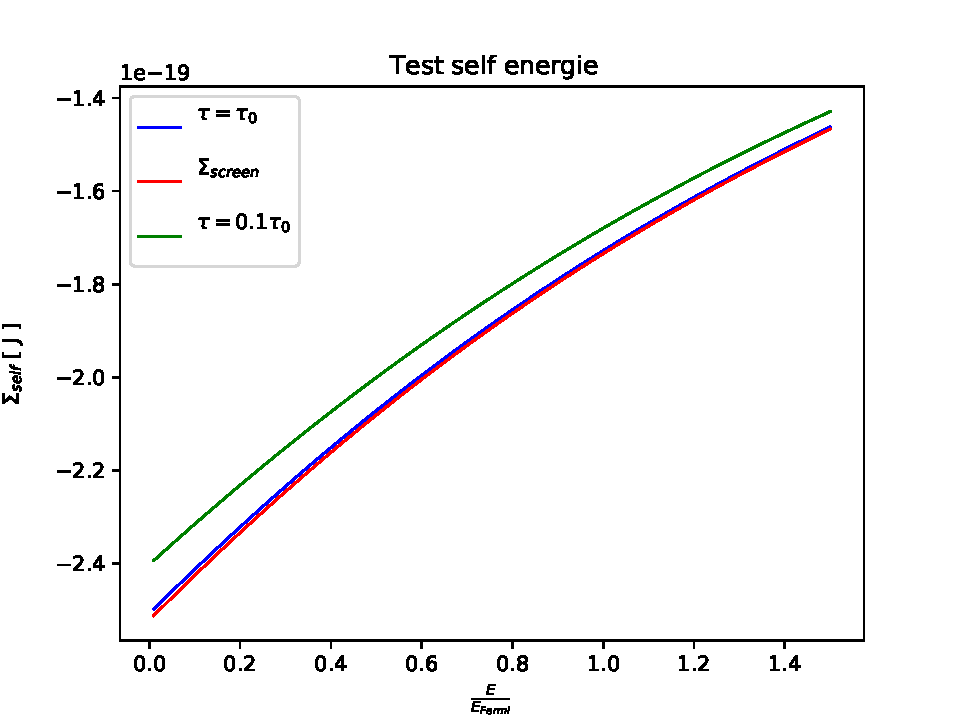
\includegraphics[scale=1]{grafy/plot_se_test}[t]
\caption{Self-energia normovaná na $\E_F$ v závislosti od energie elektrónu $\E/\E_F$, kde $\E_F=9.75$ $eV$. Prerušovaná čiara ukazuje závislosť získanú tabeláciou vzorca \eqref{eq:06fockscreen}. 
Plné čiary sú výsledky získané numerickým vypočtom vzťahu \eqref{eq:05energy6} s  $q_{max} = \infty$ (prakticky $q_{max} = 10 k_F$)  pre postupne narastajúcu
hodnotu rozptylového času $\tau$,teda pre slabší a slabší disorder. Plné čiary sa s rastúcou hodnotou $\tau$ blížia k prerušovanej čiare a pre dostatočne veľké $\tau$ sa s ňou perfektne prekrývajú. Toto 
chovanie je v súlade s očakávaním (viď text) a možno ho považovať za dôležitý test správnosti našich numerických výpočtov vzťahu \eqref{eq:05energy6}.}
\label{fig:plot_test}
\end{figure}

Nasleduje diskusia našich hlavných výsledkov, ktoré sú ukázané na obrázkoch \ref{fig:results1}, \ref{fig:results2} a \ref{fig:results3}.
Na týchto obrázkoch plotujeme hustotu stavov \eqref{eq:erg_meandis nex prepis skratka7} prepísanú v tvare relatívnej odchýlky:
\begin{equation}\label{eq:erg_hustota stavov relat}
\frac{\rho(\E) - \rho_0(\E)}{\rho_0(\E)} = - \frac{dE_{self}^{AA}(\E)}{d\E} + \frac{dE_{self}^{free}(\E)}{d\E} \text{,}
\end{equation}
Výpočty na obrázkoch \ref{fig:results1}, \ref{fig:results2} a \ref{fig:results3} sa líšia jedine hodnotou parametrov $\tau$ a $q_{max}$.

\begin{figure}
\centering
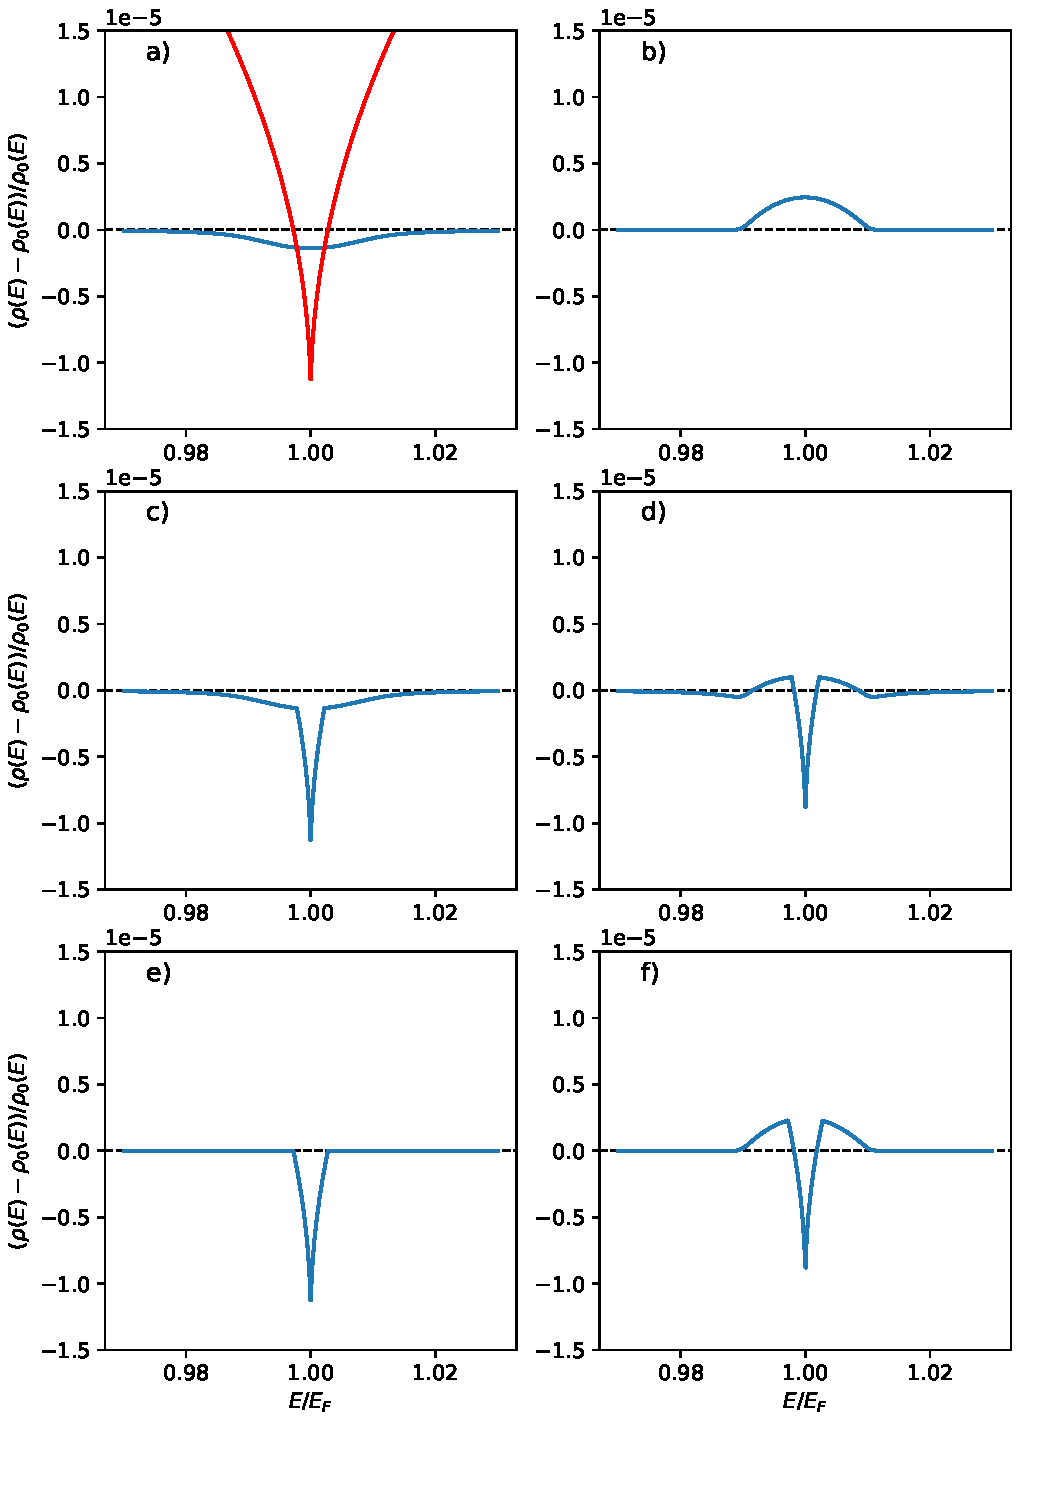
\includegraphics[scale=0.8]{grafy/plot_tau_1_c_1}[t]
\caption{Panel (a): Krivka ukázaná červenou farbou je pôvodná závislosť Altshulera - Aronova daná vzťahom \eqref{eq:erg_hustota stavov relat povodny},
krivka ukázaná modrou farbou ukazuje náš numerický výpočet vzťahu \eqref{eq:erg_hustota stavov relat naša bez}. Panel (c) ukazuje obidva grafy z panelu (a) este raz, avšak "zošité" približne v energii  $|\E-\E_F| = U_{co}$. Panel (b) ukazuje závislosť danú vzťahom \eqref{eq:erg_hustota stavov relat prvy vynech}. Panel (d) ukazuje celkovú závislosť $\frac{\rho(\E) - \rho_0(\E)}{\rho_0(\E)}$, získanú sčítaním grafov v paneloch (b) a (c).
Výpočty boli urobené pre $\tau = 6.66 \times 10^{-15} \ s$ a $q_{max} = 1/l$, ostatné parametre sú uvedené v texte.}
\label{fig:results1}
\end{figure}


Začneme grafmi na obrázku \ref{fig:results1}, vypočítanými pre $\tau = 6.66 \times 10^{-15} \ s$ a $q_{max} = 1/l$. Panel (a) na obr. \ref{fig:results1} ukazuje červenou farbou pôvodný výsledok Altshulera - Aronova 
\begin{equation}\label{eq:erg_hustota stavov relat povodny}
\frac{\rho(\E) - \rho_0(\E)}{\rho_0(\E)} = - \frac{e^{2}}{\epsilon_0 k_s^{2}}\ \  \frac{q_{max}}{2\pi^3 \hbar D}
 +  \frac{e^{2}}{\epsilon_0 k_s^{2}} \ \ \frac{1}{2\pi^2 (2\hbar D)^{3/2}}  \ \sqrt{|\E-\E_F|} \text{,}
\end{equation}
ktorý neberie do úvahy člen $\frac{dE_{self}^{free}(\E)}{d\E}$. Zopakujme, že vzťah \eqref{eq:erg_hustota stavov relat povodny}  platí pre $|\E-\E_F| \lesssim U_{co}$, kde  $U_{co} = 0.27 \frac{\hbar}{\tau}$ pre $q_{max} = 1/l$. 

Pre porovnanie, panel (a) ukazuje
aj závislosť 
\begin{equation}\label{eq:erg_hustota stavov relat naša bez}
\frac{\rho(\E) - \rho_0(\E)}{\rho_0(\E)} = - \frac{dE_{self}^{AA}(\E)}{d\E} \text{,}
\end{equation}
čo je náš výsledok \eqref{eq:erg_hustota stavov relat povodny} s vynechaným členom $\frac{dE_{self}^{free}(\E)}{d\E}$. 
Ako bolo diskutované v prechádzajúcej kapitole, náš výpočet člena  $- \frac{dE_{self}^{AA}(\E)}{d\E}$ platí pre 
$|\E-\E_F| \gtrsim \frac{\hbar}{\tau}$, pretože je založený na self-konzistentnej Bornovej aproximácii. Panel (a)
na Obr. \ref{fig:results1} ukazuje, že k určitému potlačeniu hustoty stavov v okolí Fermiho energie dochádza aj v self-konzistentnei Bornovej aproximácii.
\vspace{2cm}

Panel (c) ukazuje obidva grafy z panelu (a) este raz, avšak "zošité" približne v energii  $|\E-\E_F| = U_{co}$. Získali sme tak graf, ktorý je
kvantitatívne správny v nízkoenergetickej limite $|\E-\E_F| \ll  U_{co}$ (Altshuler-Aronovova teória) a tiež v opačnej limite $|\E-\E_F| \gg U_{co}$ (tam platí naša Bornovská teória). 
V okolí energie $U_{co}$ je získaný graf samozrejme len orientačný a kvalitatívny. Keby sa do našej Bornovskej teórie (dodatok C) pridali vyššie poruchové členy, zošitie oboch teórii v 
paneli (c) by možno bolo hladšie.

Panel (b) na obrázku \ref{fig:results1} ukazuje závislosť 
\begin{equation}\label{eq:erg_hustota stavov relat prvy vynech}
\frac{\rho(\E) - \rho_0(\E)}{\rho_0(\E)} =  \frac{dE_{self}^{free}(\E)}{d\E} \text{,}
\end{equation}
čo je závislosť \eqref{eq:erg_hustota stavov relat}, avšak s vynechaným členom $- \frac{dE_{self}^{AA}(\E)}{d\E}$.
Očividne, na rozdiel od člena $- \frac{dE_{self}^{AA}(\E)}{d\E}$, člen $\frac{dE_{self}^{free}(\E)}{d\E}$ hustotu stavov v okolí Fermiho energie zväčšuje.

Konečne, panel (d) na obr.  \ref{fig:results1} ukazuje celkovú závislosť $\frac{\rho(\E) - \rho_0(\E)}{\rho_0(\E)}$, získanú sčítaním grafov v paneloch (b) a (c).
Pri energiách $|\E-\E_F| \lesssim U_{co}$ vidíme na paneli (d) už  dobre známe potlačenie hustoty stavov podľa Altshulera a Aronova. Pre energie tesne nad $U_{co}$ však 
na paneli (d) jasne vidíme, že závislosť $\frac{\rho(\E) - \rho_0(\E)}{\rho_0(\E)}$ sa stala kladnou. Inými slovami, na paneli (d) vidíme, že pomerne významná časť stavov sa nakopila tesne nad energiou
$U_{co}$, tak ako to ukazujú experimentálne dáta na obr. \eqref{fig:B2}. 
Podobnosť teoretického grafu v paneli (d) obrázku ref{fig:results1} a experimentálnych grafov na obr. \eqref{fig:B2} je podľa nášho názoru pozoruhodná.

Náš teoretický graf v paneli (d) obrázku ref{fig:results1} ukazuje pre dostatočne veľké energie nad $U_{co}$ aj jemný prepad do záporných hodnôt. Tento jemný prepad je 
podľa nášho názoru artefakt toho, že používame ostrý cutoff $q_{max}$. Veríme, že keby sa použil hladký cutoff $e^{q/q_{max}}$, tak pozorovaný jemný prepad do záporných hodnôt by vymizol.
\vspace{5cm}



\begin{figure}[t]
\centering
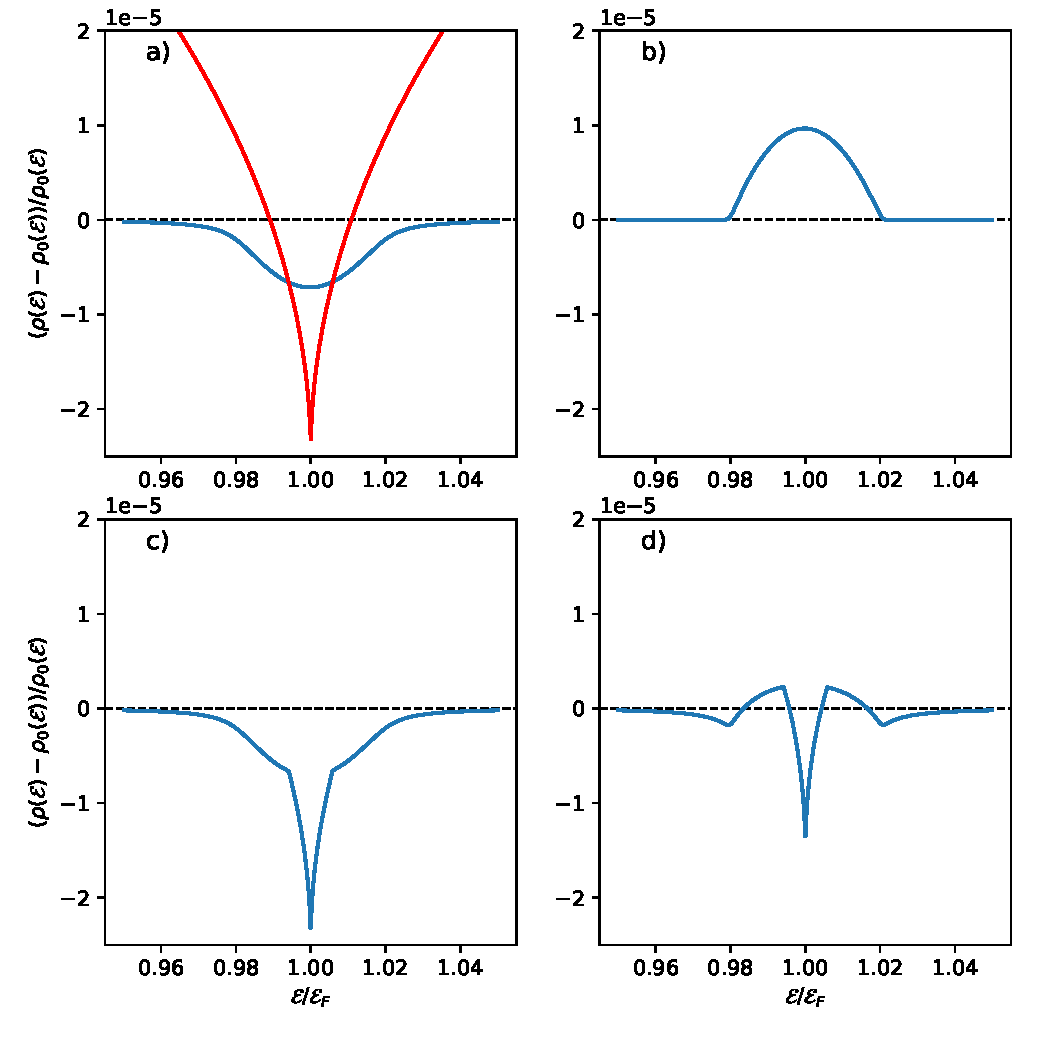
\includegraphics[origin=c,scale=0.6]{grafy/plot_tau_1_c_1_98}
\caption{Tie isté výpočty ako na obrázku \ref{fig:results1}, len namiesto $q_{max} = 1/l$ sme použili $q_{max} = 1.92/l$. }
\label{fig:results2}
\end{figure}

\begin{figure}[H]
\centering
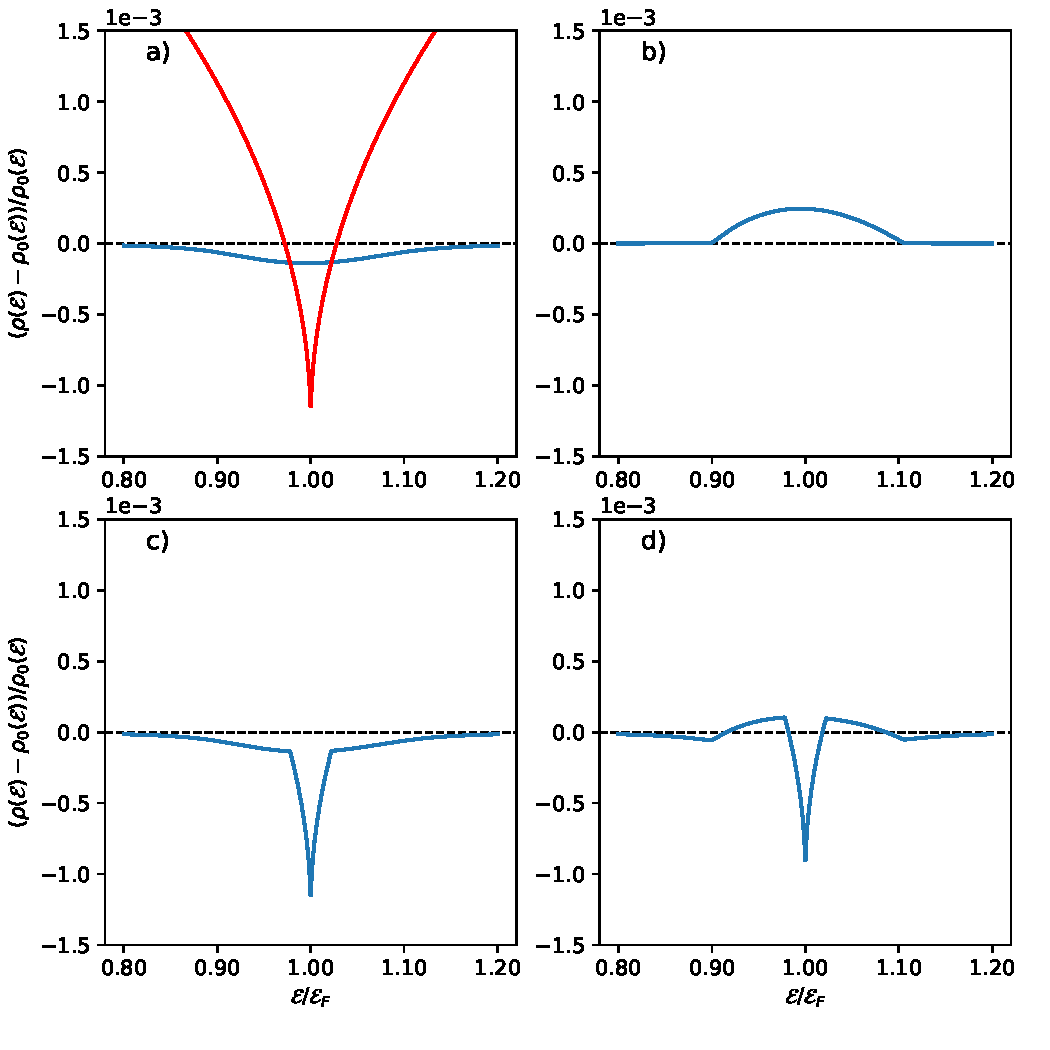
\includegraphics[origin=c,scale=0.6]{grafy/plot_tau_0_1_c_1}
\caption{Tie isté výpočty ako na predchádzajúcich dvoch obrázkoch, avšak pre  $\tau = 6.66 \times 10^{-16} \ s$ a $q_{max} = 1/l$.}
\label{fig:results3}
\end{figure}


